\documentclass[./dissertation.tex]{subfiles}

\begin{document}
    
    \contentchapter{Results}
    
    \section{General Experimental Configuration}
    Each set of experiments shares a common hyperparameter search space. Below we describe the fixed values or sets of values that are included in the search space of each experiment. 
    \subsection{Learning Rate}
    Through informal experimentation, we have found that the learning rate of 0.001 causes the models to converge quickly most consistently. The learning rate is thus set to 0.001 in each experiment.
    \subsection{Latent Space Dimensionality}
    Latent space dimensionality refers to the dimensionality of the vector output of the encoder of a DML network or the dimensionality of the posterior distribution of a VAE (also the dimensionality of the latent space). We use the set containing 2 and 10 as potential values for latent space dimensionality. When the latent space dimensionality is 2, we see the added benefit of creating plots of the latent representations (though we can accomplish this through using dimensionality reduction methods like tSNE for higher dimensionalities as well).
    \subsection{Alpha}
    Alpha ($\alpha$) is a hyperapameter which refers to the balance between the unsupervised and supervised losses of some of the modified DML models. More details about the role of $\alpha$ in the model implementations are discussed in the methodology section of the model. We iterate through the set containing 0.25, 0.5, 0.75, 1, which represent 25\% increments in the balance between the unsupervised and supervised loss in semi-supervised training. We do not include 0 in this set as if $\alpha$ is set to 0, the model is equivalent to the fully supervised plain DML model because the supervised loss would not be included.
    \subsection{Partial Labels Percentage}
    The partial labels percentage hyperparameter refers to the percentage of the dataset that is labelled and thus the size of the partion of the dataset that can be used for labelled training. Of course, each of the datasets we use is fully labelled, so a partially labelled datset can be trivially constructed by ignoring some of the labels. As the sizes of the dataset vary, each percentage can refer to a different number of labelled samples. We iterate through the set containing 0.01, 0.1, 1, 10, 100, for this hyperparameter (with each value referring to the percentage). 
    \subsection{Datasets}
    Two datasets are used for evaluating the models. The first dataset is MNIST (\cite{lecun-mnisthandwrittendigit-2010}), a very popular dataset containing greyscale images of handwritten digits. The second dataset we use is the organ OrganAMNIST dataset from MedMNIST v2 (\cite{medmnistv2}). This dataset contains 2D slices from computed tomography images from the Liver Tumor Segmentation Benchmark -- the labels correspond to the classification of 11 different body organs. The decision to use a second dataset was motivated because the as the claims are tested over more datasets, the claims themselves are more generalizable. The decision to use the OrganAMNIST datasets specifically is motivated in part due to the the Quinn Research Group working on similar tasks for biomedical imaging (\cite{Zain2020TowardsAU}). It is also motivated in part because OrganAMNIST is a more difficult dataset, at least for a the classfication task, as the leading accuracy for MNIST is .9991 (\cite{DBLP:journals/corr/abs-2008-10400}) while the leading accuracy for OrganAMNIST is .951 (\cite{medmnistv2}). The MNIST and OrganAMNIST datasets are similar in dimensionality (1 x 28 x 28), number of samples (60,000 and 58,850, respectively) and in that they are both greyscale.
    
    \begin{figure}[h]
        \centering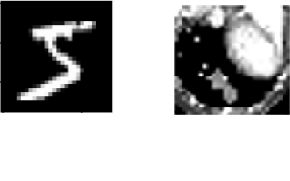
\includegraphics[width=0.5\textwidth]{figures/cropped_datasets.png}
        \caption{Sample images from the MNIST (left) and OrganAMNIST of MedMNIST (right) datasets}
        \label{Datasets Diagram}
    \end{figure}
    
    \subsection{Evaluation}
    We will evaluate the results by running each model on a test partition of data. We then take the latent points $Z$ generated by the model and the corresponding labels $Y$. Three classifiers (sklearn's implementation of RandomForest, MLP, and kNN) each output predicted labels $\hat{Y}$ for the latent points. We finally measure the quality of the predicted labels $\hat{Y}$ using the Adjusted Mutual Information Score (AMI) (\cite{vinh2010information}) and accuracy (which is still helpful but is also easier to interpret in some cases). This scoring metric is common in research that looks to evaluate clustering performance \cite{zhu2021finding} \cite{emmons2016analysis}). We will be using sklearn's implementation of AMI \cite{scikit-learn}. The performance of a classifier on the latent points intuitively can be used as a measure of quality of clustering.
    \section{Claim 1: Benefits of Reconstruction Loss}
    In evaluating the first claim, we compare the performance of the plain DML model to the DML Autoencoder model. We do so by comparing the performance of the plain DML system and the DML Autoencoder across the specified set of hyperparameters (including datasets).
   \begin{table}[]
       \centering
       \begin{tabular}{|c|c|c|c|}
            \hline
            \textbf{pl\%} & \textbf{lsdim} & \textbf{knn acc} & \textbf{knn MI}  \\
            \hline
            0.01 & 2 & 0.2603 & \textbf{0.1163} \\
            & & & \\ 
            & & & \\ 
            & & & \\ 
            & 10 & \textbf{0.2678} & 0.1126 \\ 
            & & & \\ 
            & & & \\ 
            & & & \\ 
            0.1 & 2 & 0.4247 & 0.2916 \\
            & & & \\ 
            & & & \\ 
            & & & \\ 
            & 10 & \textbf{0.6577} & \textbf{0.5005} \\ 
            & & & \\ 
            & & & \\ 
            & & & \\
            10 & 2 & 0.7450 & 0.6156 \\
            & & & \\ 
            & & & \\ 
            & & & \\ 
            & 10 & \textbf{0.9466} & \textbf{0.8753} \\ 
            & & & \\ 
            & & & \\ 
            & & & \\
            \hline
       \end{tabular}
        \begin{tabular}{|c|c|c|c|c|}
            \hline
            \textbf{pl\%} & \textbf{alpha} & \textbf{lsdim} & \textbf{knn acc} & \textbf{knn MI}  \\
            \hline
            0.01 & 0.25 & 2 & 0.4010 & 0.2847 \\
             &  & 10 & 0.8251 & 0.7070 \\
             & 0.5 & 2 & 0.3314 & 0.1881 \\
             &  & 10 & 0.6688 & 0.5216 \\
             & 0.75 & 2 & 0.3107 & 0.1878 \\
             &  & 10 & \textbf{0.8347} & 0.7054 \\
             & 1 & 2 & 0.4115 & 0.2894 \\
             &  & 10 & 0.8377 & \textbf{0.7182} \\
            0.1 & 0.25 & 2 & 0.4322 & 0.3329 \\
             &  & 10 & 0.8761 & 0.7676 \\
             & 0.5 & 2 & 0.4169 & 0.3166 \\
             &  & 10 & \textbf{0.8881} & \textbf{0.7856} \\
             & 0.75 & 2 & 0.3638 & 0.2649 \\
             &  & 10 & 0.7891 & 0.6483 \\
             & 1 & 2 & 0.4157 & 0.2947 \\
             &  & 10 & 0.8560 & 0.7408 \\
            10 & 0.25 & 2 & 0.1013 & 0 \\
             &  & 10 & 0.8518 & 0.7273 \\
             & 0.5 & 2 & 0.3440 & 0.2199 \\
             &  & 10 & 0.7912 & 0.6556 \\
             & 0.75 & 2 & 0.3512 & 0.2153 \\
             &  & 10 & \textbf{0.8533} & \textbf{0.7418} \\
             & 1 & 2 & 0.5155 & 0.3741 \\
             &  & 10 & 0.8494 & 0.7277 \\
            \hline
       \end{tabular}
       \caption{Comparison of the DML (left) and MetricAutoencoder (right) models for the MNIST dataset. Bolded values indicate best performance for each partial labels percentage partition (pl\%).\\}
       \label{tab:my_label}
   \end{table}
   In table 1.1, we observe that for relatively small amounts of labelled samples (the partial labels percentages of 0.01 and 0.1 correspond to 6 and 60 labelled samples respectively), the Metric Autoencoder severely outperforms the DML model. However, when the number of labelled samples increases (the partial labels percentage of 10 correspond to 6000 labelled samples respectively), the DML model significantly outperforms the metric autoencoder. This trend is not too suprising, as when there is sufficient data to train unsupervised methods and insufficient data to train supervised method, as is the case for the 0.01 and 0.1 partial label percentages, the unsupervised method will likely perform better. \\
   
   It is somewhat surprising is that the injection of labelled data does not appear to definitively improve the performance of the Metric Autoencoder, as evidenced by the comparing $\alpha=1$ to other values of $\alpha < 1$ that incorporate metric loss into the overall loss and as evidenced by the increasing percentage of labelled data having little effect on performance. \\ 
   
   In observing the other hyperparameters, we see that for almost every model configuration, setting the latent space dimensionality to 10 dimensions (as opposed to 2 dimensions) causes a significant increase in performance. This is not surprising as the representational power of the latent space grows with its dimensionality. It is difficult to assess the role of alpha in the Metric Autoencoder with regards to model performance. \\
   
   The data looks to show that the claim that adding a reconstruction loss to a DML system can improve the quality of clustering in the latent representations on a semi-supervised dataset when there are small amounts (roughly less than 100 samples) of labelled data \textit{and} a sufficient quantity of unlabelled data. But an important caveat is that it is not convincing that the metric autoencoder effectively combined the unsupervised and supervised losses to create a superior model, as a plain autoencoder (i.e. the Metric Autoencoder with $\alpha = 1$) outperforms the DML for the partial labels percentage of or less than 0.1\% and underperforms the DML for the partial labels percentage of 10\%. \\
   
   TODO: Make and Discuss results for MedMNIST dataset
    \section{Claim 2: Incorporating Inductive Bias with Prior}
    In evaluating the second claim, we compare the performance of the plain DML model to the DML with a unit prior and a DML with a GMM prior. We also compare the performance to a DML with a VampPrior. Gaging the performance of a DML with a learnable prior like a VampPrior is not as key to evaluating whether inductive bias can be incorporated because the VampPrior not only incorporates inductive bias but adds complexity, while the unlearned priors only incorporate inductive bias. However, we still run experiments with the DML with VampPrior as we feel it is in line with this thesis' goals to assess how components of VAE and modified VAE models can augment and improve the standard DML model. \\ 
    - Assign each cluster to a psuedoinput using KNN. Then plot the percentages of each class within each pseudoinput for each pseudoinput. Measure the homogenity for each pseudoinput to see if relationship between that and mutual inforamtion score.
    \section{Claim 3: Jointly Optimizing DML with VAE}
    - DML vs VAE vs VAE Auteoncoder \\
    - Different Losses
    
    
\end{document}
